\chapter{METHODOLOGY}\label{chp:Methodology}

Correspondingly, this chapter discusses the approaches for detecting pes cavus and pes planus, and as well as machine learning.

\section{FOOT DEFORMITY DETECTION} \label{sec:MethodologyFootDeformityDetection}

One of the most efficient techniques to detect pes planus and pes cavus is using radiological scans. On the other hand, Pes planus and pes cavus may only be seen when the feet are pressed on the sole. Thereby, lateral radiographs are taken laterally or from the top of the knee and downwards for arch measures, while pushing the foot on the ground.

Many approaches for determining the state of the foot using radiological imaging have been documented in the literature. Calcaneal inclination angle, first metatarsal declination angle, lateral talocalcaneal angle, and Meary's angle are the most well-known of them all.

\begin{figure}[htbp]
\centering
\fbox{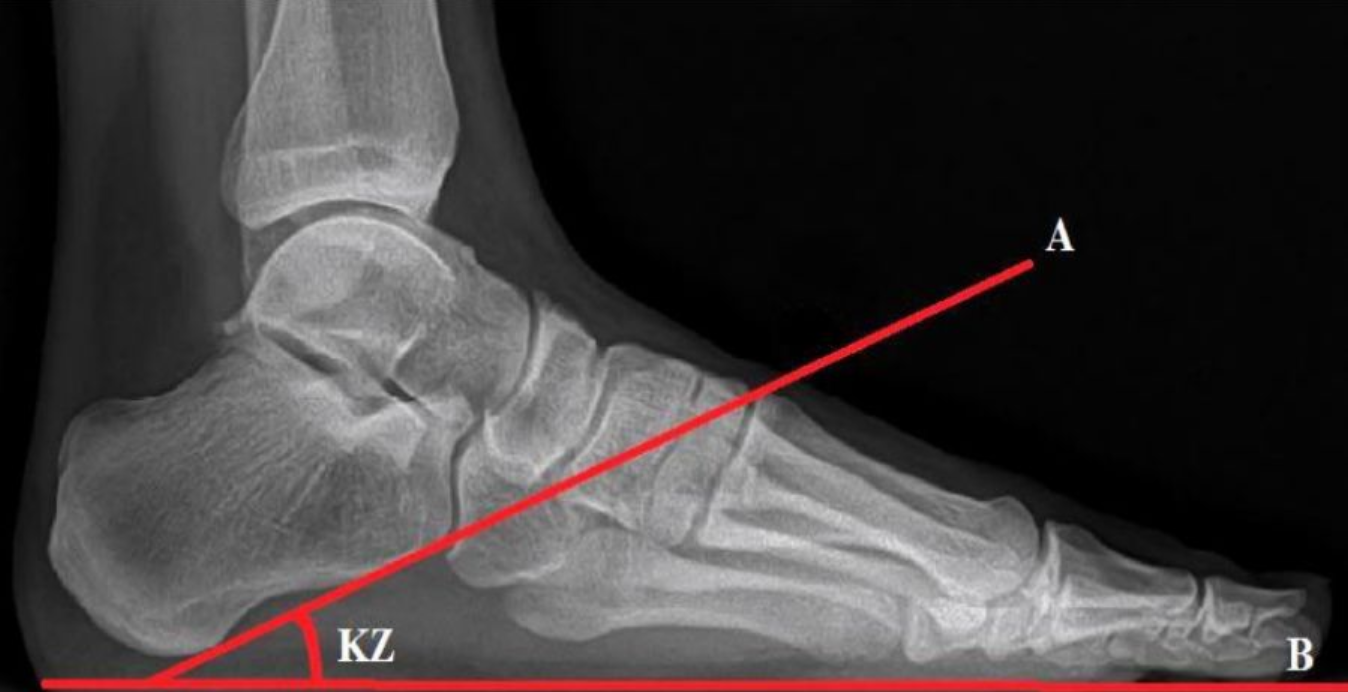
\includegraphics[width=.6\columnwidth]{KaanEksenMSc/figures/MethodologyCalcaneusInclinationAngle.png}}
\caption{Calcaneus Inclination Angle \cite{deniz2014ccocuklardaki}}
\label{fig:MethodologyCalcaneusInclinationAngle}
\end{figure}

The angle formed by a tangent line drawn between the lower face of the calcaneus to the ground is known as the calcaneus inclination angle ( see Figure \ref{fig:MethodologyCalcaneusInclinationAngle}) \cite{deniz2014ccocuklardaki}. If the calcaneal inclination angle is between 20 and 25 degrees, the foot is considered healthy. Pes planus, on the other hand, is defined as an angle of fewer than 15 degrees \cite{flores2019adult}. However, if the angle is more than 30 degrees, it is considered pes cavus \cite{yates2009merriman}.

\begin{figure}[htbp]
\centering
\fbox{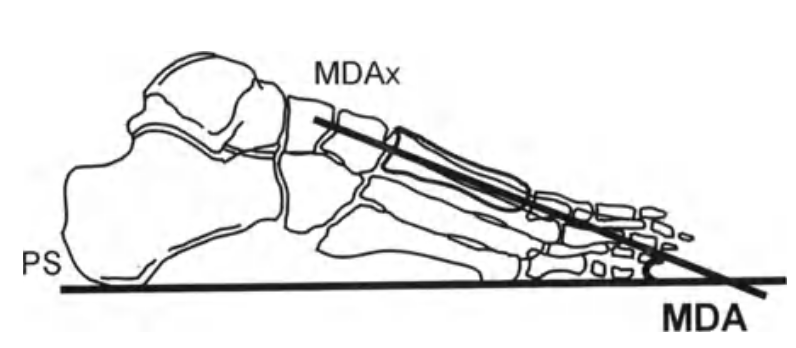
\includegraphics[width=.6\columnwidth]{KaanEksenMSc/figures/MethodologyMetatarsalDeclinationAngle.png}}
\caption{Metatarsal Declination Angle \cite{davies2012imaging}}
\label{fig:MethodologyMetatarsalDeclinationAngle}
\end{figure}

The metatarsal declination angle is measured by considering the horizontal surface under the sole and the calcaneal inclination axis and using a weight-bearing lateral foot radiograph (see Figure \ref{fig:MethodologyMetatarsalDeclinationAngle}). The metatarsal declination angle in the general population is predicted to be around 21 degrees [33]. In any situation, the metatarsal declination angle is greater than 30 degrees, defined as pes planus [33].

\begin{figure}[htbp]
\centering
\fbox{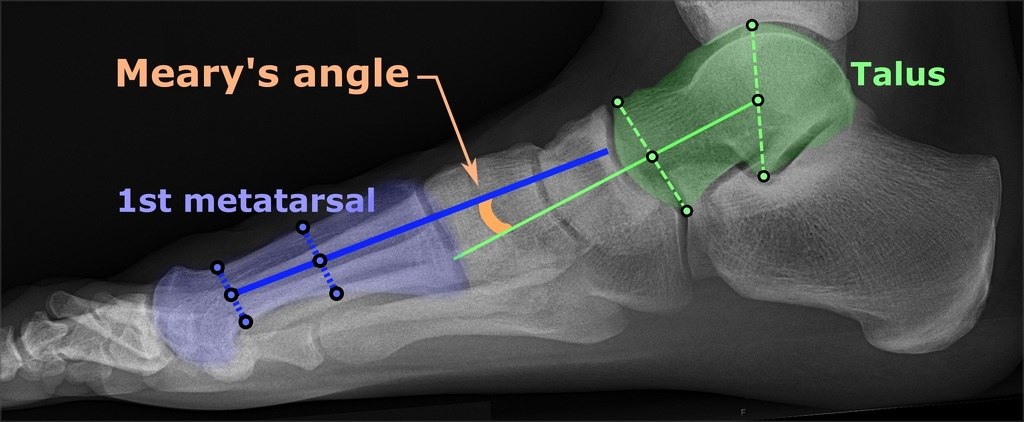
\includegraphics[width=.6\columnwidth]{KaanEksenMSc/figures/MethodologyMearysAngle.jpg}}
\caption{Meary's Angle \cite{radiopaediamearysangle}}
\label{fig:MethodologyMearysAngle}
\end{figure}

Meary's angle \cite{deniz2014ccocuklardaki} is calculated by drawing a line through the centers of the longitudinal axes of the talus and first metatarsal (see Figure \ref{fig:MethodologyMearysAngle}). The foot is designated pes planus if the resulting angle is more than 4 degrees (convex downward) \cite{vanderwilde1988measurements}. If the computed angle is less than -4 degrees (convex upward), the foot is classified as pes cavus \cite{banks2001mcglamry}.

\begin{figure}[htbp]
\centering
\fbox{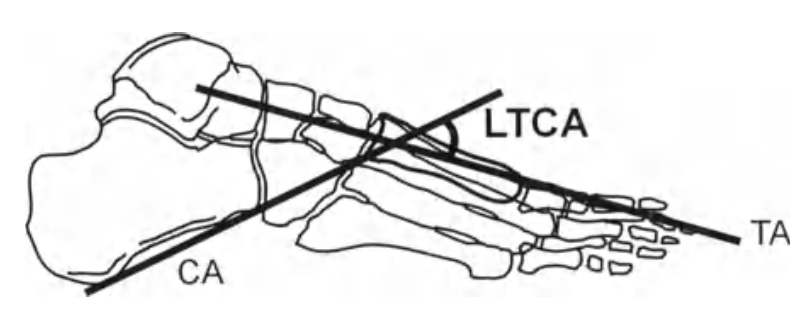
\includegraphics[width=.6\columnwidth]{KaanEksenMSc/figures/MethodologyLateralTalocalcanealAngle.png}}
\caption{Lateral Talocalcaneal Angle \cite{radiopaediamearysangle}}
\label{fig:MethodologyLateralTalocalcanealAngle}
\end{figure}

The calcaneal axis and the collum lateral axis form the lateral talocalcaneal angle (see Figure \ref{fig:MethodologyLateralTalocalcanealAngle}) in a weight-bearing lateral foot radiograph.  If the angle is less than 35 degrees, it is considered pes cavus.  In contrast, if the angle is more than 50 degrees, it is diagnosed as pes cavus.

Compared to the anthropometric pes planus and cavus detection procedures stated above, non-anthropometric measurements, while less accurate, are significantly more readily available, less expensive to do, and less harmful - i.e., do not require people to expose themselves to radiation. Therefore, Non-anthropometric procedures can be performed in large groups and in advance due to their ease of access.

The footprint approach, which involves sinking the foot into ink and then pressing it onto graph paper, is one of the most common non-anthropometric methods used in the literature. Many indexes, such as the Staheli arch and the Chippaux-Smirak indices, use graph paper to identify pes planus and pes cavus.

\begin{figure}[htbp]
\centering
\fbox{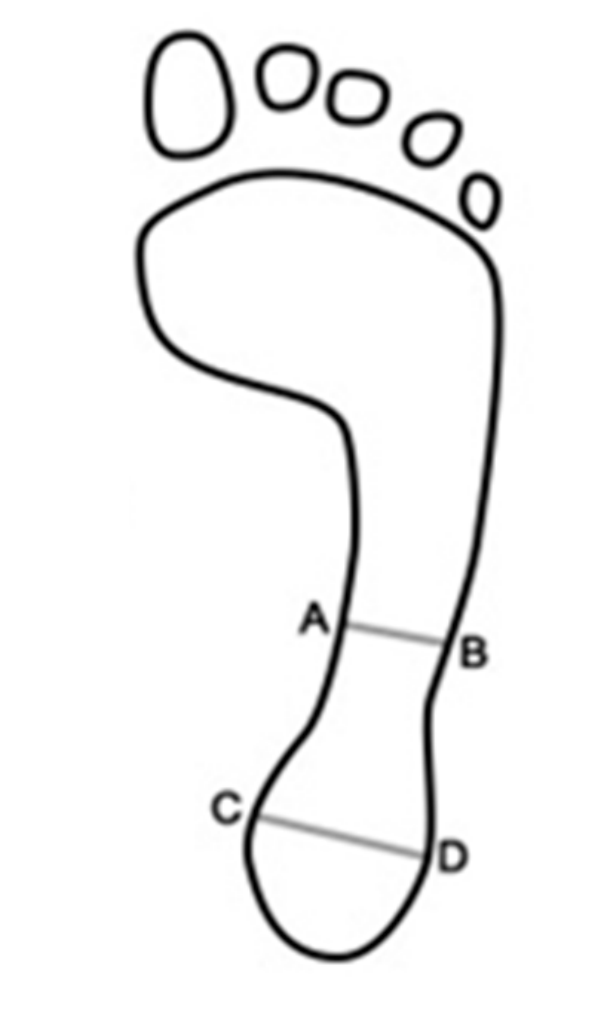
\includegraphics[width=.2\columnwidth]{KaanEksenMSc/figures/MethodologyStaheliIndex.png}}
\caption{Staheli Index AB/CD \cite{radiopaediamearysangle}}
\label{fig:MethodologyStaheliIndex}
\end{figure}

By dividing the width of a foot's center part by the width of the heel region, the Staheli index is determined (see Figure \ref{fig:MethodologyStaheliIndex}). The foot is considered pes planus if the determined ratio (index) is more than 0.8. However, if the estimated ratio is less than 0.4, it is classified as pes cavus \cite{almaawi2019flatfoot}.

\begin{figure}[htbp]
\centering
\fbox{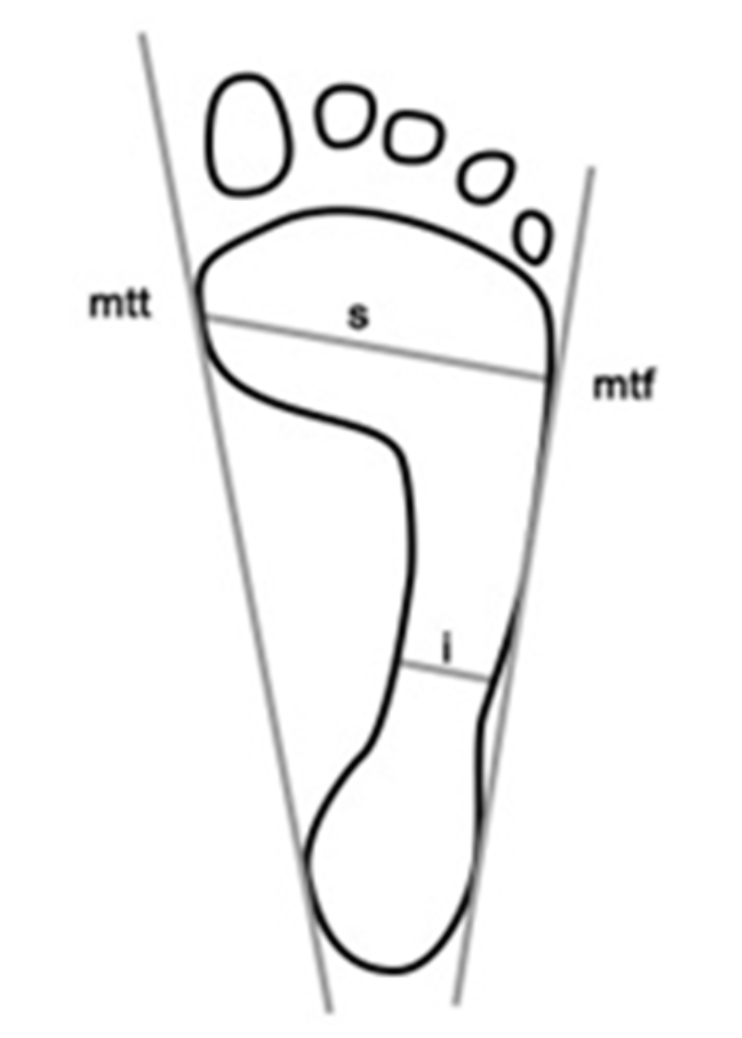
\includegraphics[width=.25\columnwidth]{KaanEksenMSc/figures/MethodologyChippauxSmirakaIndex.png}}
\caption{Chippaux-Smiraka Index i/s \cite{radiopaediamearysangle}}
\label{fig:MethodologyChippauxSmirakaIndex}
\end{figure}

The Chippaux-Smirak Index (see Figure \ref{fig:MethodologyChippauxSmirakaIndex}) is calculated by taking into account the ratio of the midfoot's narrowest and widest regions. Therefore resulting proportion greater than 0.45 in the Chippaux-Smirak Index is defined as Pes planus. On the other hand, it is considered pes cavus\cite{almaawi2019flatfoot} if the proportion is less than 0.25.

\begin{figure}[htbp]
\centering
\fbox{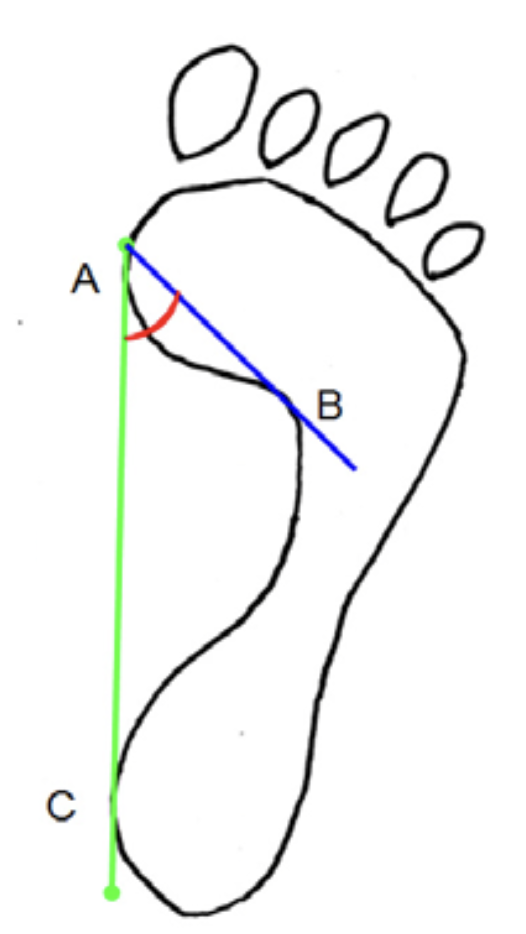
\includegraphics[width=.25\columnwidth]{KaanEksenMSc/figures/MethodologyClarkesAngle.png}}
\caption{Clarke's Angle \cite{ozer2012evaluation}}
\label{fig:MethodologyClarkesAngle}
\end{figure}

The Clarke angle is formed by the line joining the tangent at the medial edge (A-C line in Figure \ref{fig:MethodologyClarkesAngle}) of the footprint and the longest vertical distance from the medial border of the foot to the point where the medial tangent intersects the edge of the forefoot(A-B line in Figure \ref{fig:MethodologyClarkesAngle}). Normal (42°–54°), mild flatfoot (35°–41°), moderate flatfoot (30°–34.9°), severe flatfoot (30°), and high arched foot ($>$ 54°) are the classifications for Clarke's angle \cite{hegazy2021comparing}.

\begin{figure}[htbp]
\centering
\fbox{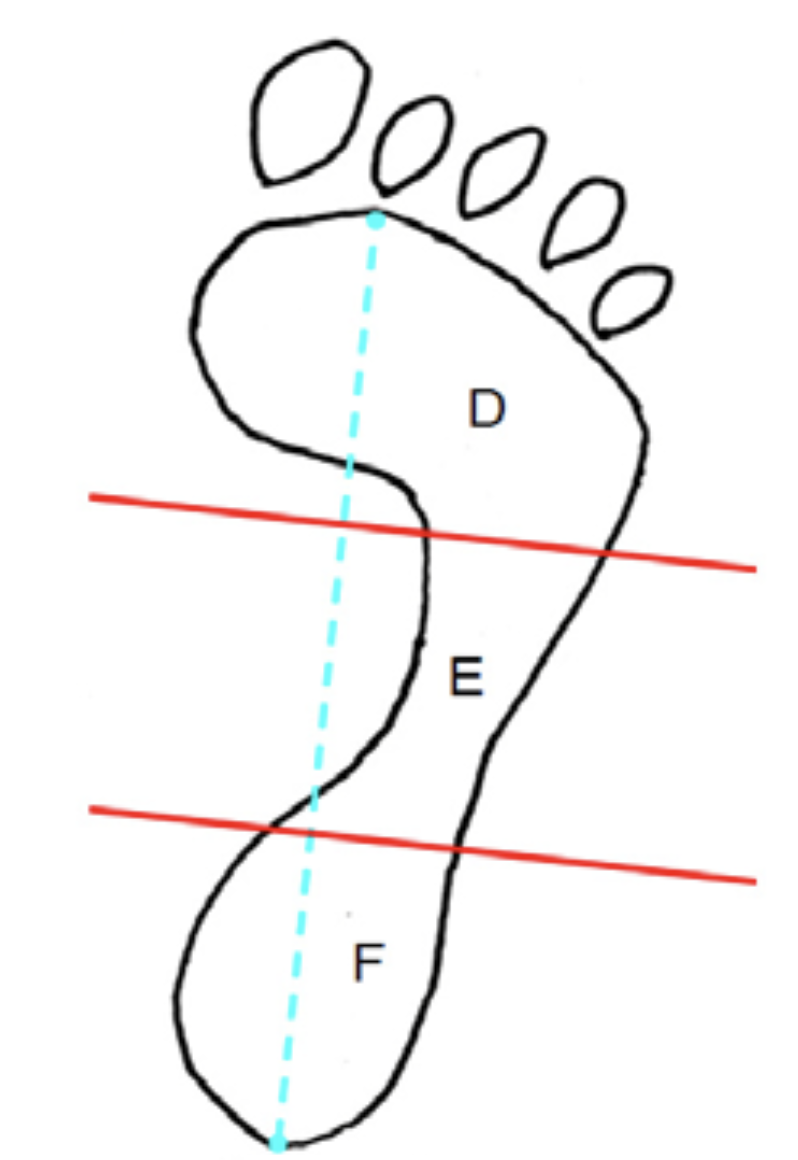
\includegraphics[width=.25\columnwidth]{KaanEksenMSc/figures/MethodologyArchIndex.png}}
\caption{Arch Index E/D+E+F \cite{ozer2012evaluation}}
\label{fig:MethodologyArchIndex}
\end{figure}

The arch index is calculated by the midfoot area (E in Figure \ref{fig:MethodologyArchIndex}) in ratio to the sum of the hindfoot (F in Figure \ref{fig:MethodologyArchIndex}), midfoot, and forefoot (D in Figure \ref{fig:MethodologyArchIndex}) areas. If the ratio of the arch index is equal to or larger than 0.26, it is considered flat foot. If it is less than 0.21, it is considered pes cavus. Otherwise, it is a normal arch \cite{igbigbi2005arch}. 

\begin{figure}[htbp]
\centering
\fbox{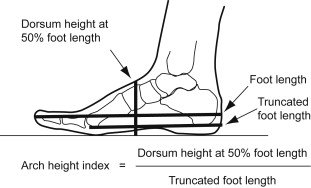
\includegraphics[width=.50\columnwidth]{KaanEksenMSc/figures/MethodologyArchHeightIndex.png}}
\caption{Arch Index E/D+E+F \cite{miller2014effect}}
\label{fig:MethodologyArchHeightIndex}
\end{figure}

There are other non-anthropometric procedures without using the footprint, such as arch height and rearfoot angle. Instead, they are using intermediate results such as pictures to make measurements.

The arch height at 50 \% of the entire foot length is divided by the truncated foot length to calculate the arch height index (see Figure \ref{fig:MethodologyArchHeightIndex}). In the arch height index average pes planus value is 0.35 ± 0.03 and average pes cavus is 0.40 ± 0.03 \cite{hillstrom2013foot}.

\begin{figure}[htbp]
\centering
\fbox{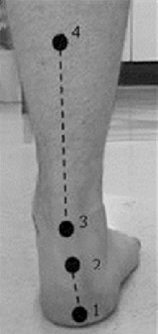
\includegraphics[width=.40\columnwidth]{KaanEksenMSc/figures/MethodologyRearfootAngle.jpg}}
\caption{Rearfoot angle critical points \cite{langley2016clinical}}
\label{fig:MethodologyRearfootAngle}
\end{figure}

Rearfoot angle is calculated using the angle between two lines, As illustrated in the figure \ref{fig:MethodologyRearfootAngle}. The lines contracted by the four points are the Achilles tendon center at the height of medial malleoli, Achilles tendon center at the height of medial malleoli, the center of shank posterior, 15 cm above the Achilles tendon center, and the base of the calcaneus \cite{huerta2008relationship}. If the calculated angle is between -4 and 4 degrees, the foot is classified as normal. On the other hand, If the computed angle is larger than 5 degrees and valgus, it is considered pes planus. If it is then 5 degrees and varus, it is classified as pes cavus \cite{jonson1997intraexaminer}.

\section{DEEP LEARNING}

Deep learning is a prominent object identification approach, a subset of machine learning that can be supervised (such as classification) or unsupervised. As a result, deep learning employs a large number of non-linear processing unit layers for feature extraction and conversion. Hence, each subsequent layer uses the output of the preceding layer as input and produces a classification \cite{goodfellow2016deep}.

One of the most influential aspects of deep learning is feature extraction. Low and high level (i.e., features extracted from low-level features)
can be automatically extracted from data in deep learning. Therefore, manual features extraction has become obsolete in deep learning. However, deep learning algorithms require comprehensive data and high-performance hardware to process this data compared to other machine learning algorithms \cite{lecun2015deep}.

Deep learning is a very effective method that provides the ability to train and learn systems with large and complex probabilistic models. In order to achieve this, it uses different layers in a data representation. Therefore this provides the ability to be pre-trained those layers separately. As a result, recent research shows that it provides more successful results than traditional approaches \cite{chen2015net2net, huang2013cross}.

The data's size and complexity are significant factors in deep learning training. Therefore, increased complexity and size affect the training time. Transfer learning can be used to reduce training time by using deep learning algorithms trained in similar fields \cite{goodfellow2016deep}. 

There are many deep learning architectures. Some of the significant architectures will be discussed in the following paragraphs starting with artificial neural networks such as artificial neural network, recurrent neural networks, convolutional neural networks. 

Artificial neural networks are a building block of deep learning that performs functions such as remembering, learning, generalizing, and producing new information by mimicking the human brain. Artificial neural networks are used in many fields and applications such as classification, modeling, and prediction, and they are improving day by day, such as fingerprint recognition \cite{baldi1993neural}, autonomous vehicles \cite{tian2018deeptest}, voice recognition \cite{melin2006voice}, meteorological interpretation \cite{hsieh1998applying}, handwriting recognition\cite{oh2002class}.

\begin{figure}[htbp]
\centering
\fbox{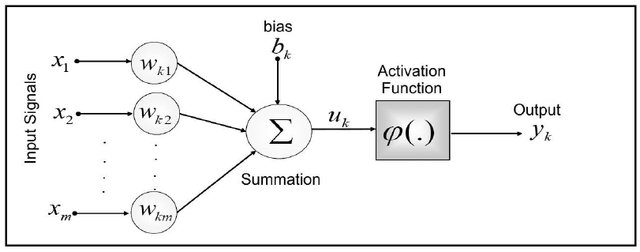
\includegraphics[width=.60\columnwidth]{KaanEksenMSc/figures/MethodologyArtificialNeural.jpg}}
\caption{Artificial neural \cite{veronez2011regional}}
\label{fig:MethodologyArtificialNeural}
\end{figure}

Artificial neurons have a straightforward structure. It consists of input, weights, bias, activation function, and output (see Figure \ref{fig:MethodologyArtificialNeural}). Inputs are data coming into neurons from another artificial neuron or the initial input. The input is multiplied by a weight value and summed with the bias, which is optional. Therefore, each input effect can be adjusted. After calculating the value, the output is produced with the help of the activation function. 

\begin{figure}[htbp]
\centering
\fbox{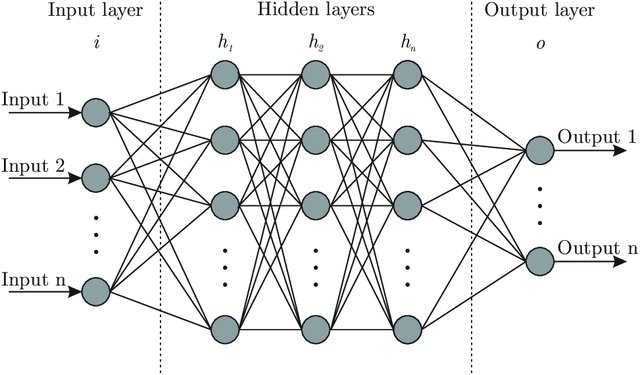
\includegraphics[width=.60\columnwidth]{KaanEksenMSc/figures/MethodologyArtificialNeuralNetwork.jpg}}
\caption{Artificial neural \cite{bre2018prediction}}
\label{fig:MethodologyArtificialNeuralNetwork}
\end{figure}

The combination of artificial neurons cells forms artificial Neural Networks. Artificial Neural Networks are examined in three main layers. These are the input layer, hidden layers, and output layer (see Figure \ref{fig:MethodologyArtificialNeuralNetwork}). The input layer brings the initial data into the system, which does not experience any processing and is transmitted directly to the lower layers. Furthermore, the data for further processing is transferred into the hidden layer. Depending on the structure of artificial neural networks, the number of hidden layers may vary. Finally, after the processing, the output layer produces the final results. 

The calculated output and expected output values are calculated according to the error function. Therefore, the error value is the difference between the calculated output and expected values. Finally, the calculated error value is updated using the optimization function. Different parameters directly affect the success of artificial neural networks, such as the number of data, the number of layers in the neural network, the activation function, and the learning rate \cite{goodfellow2016deep}.

Recurrent neural networks (RNN) are another essential architecture with an internal memory structure. This internal structure provides input history so that it correctly predicts the future. In traditional neural networks, all input data is assumed to be independent of each other. The basic idea of recurrent neural networks is to use sequential information \cite{medsker1999recurrent}. Although RNNs are considered to be able to use information in very long sequences, in theory, it is known that returning to information is very limited in practice \cite{medsker1999recurrent}.

\begin{figure}[htbp]
\centering
\fbox{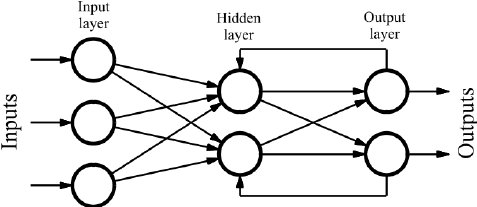
\includegraphics[width=.60\columnwidth]{KaanEksenMSc/figures/MethodologyRecurrentNeuralNetwork.jpg}}
\caption{Artificial neural \cite{quiza2009computational}}
\label{fig:MethodologyRecurrentNeuralNetwork}
\end{figure}

RNNs create a loop and use past data, which can be seen in Figure \ref{fig:MethodologyRecurrentNeuralNetwork}. RNNs are used in language modeling \cite{mikolov2011extensions}, machine translation \cite{cho2014learning}, speech recognition\cite{miao2015eesen}, image description creation \cite{mao2014deep}, and video tagging \cite{garg2021video}. 

\begin{figure}[htbp]
\centering
\fbox{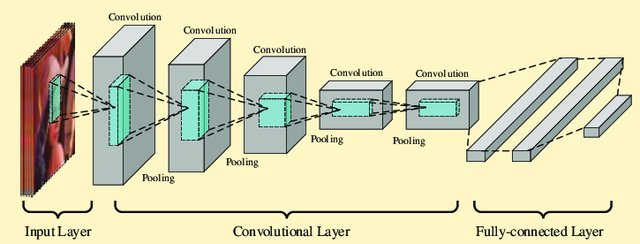
\includegraphics[width=.60\columnwidth]{KaanEksenMSc/figures/MethodologyConvolutionalNeuralNetworkExample.jpg}}
\caption{Convolutional neural network example \cite{ferracuti2019business}}
\label{fig:MethodologyConvolutionalNeuralNetworkExample}
\end{figure}

Convolutional neural networks, created by modeling the human vision system, have achieved significant success in computer vision \cite{gu2018recent, bouvrie2006notes, lavin2016fast}. It is used in many areas such as object recognition, object classification, object tracking, sentence modeling. CNN may contain many layers: the input layer, convolution layer, ReLu, pooling layer, fully connected layer, dropout layer, classification layer, and output layer (see Figure \ref{fig:MethodologyConvolutionalNeuralNetworkExample}).

The convolution layer, also known as the transform layer, is based on circulating a filter over all the input data. Filter sizes can be in different sizes such as 2x2, 3x3. The filters take the output data from the previous layer, apply the convolution operation and generate an feature map. Feature maps are regions where features specific to each filter are discovered. Edge information can also be found in this feature map \cite{goodfellow2016deep}

The convolution layer, also known as the transform layer, circulates a filter over all the input data. Filter sizes can be in different sizes, such as 2x2, 2x3. The filters take the output data from the previous layer, apply the convolution operation and generate a feature map. Feature maps are regions where features specific to each filter are discovered. Edge information can also be found in this feature map \cite{goodfellow2016deep}.

The primary purpose of the pooling layer is to reduce the size of the input data. As a result of this layer, there will be a decrease in size, and information loss will occur. This loss benefits the neural network as it reduces the computational load and prevents the system from memorizing \cite{goodfellow2016deep}.

The dropout layer is used to prevent the network from memorizing input data. Therefore removing some of the data in layers prevent this memorization. Moreover, A fully connected layer is linked to all areas of the previous layer, used in many network designs. Finally, the multidimensional data is converted to one dimension in the classification layer using the flatten method. As a result, the classification process is performed in the one-dimensional data \cite{goodfellow2016deep}.

There are many object detection applications in areas such as people counting \cite{nogueira2019retailnet}, autonomous vehicles \cite{rausch2017learning}, and face detection \cite{yang2015facial}. The general purpose of object detection is to recognize a previously defined object class in a new image and define the positions of each object it detects in this image using a rectangle that encloses the entire object \cite{goodfellow2016deep}.

Many accurate and fast algorithms are available for object detection and tracking. However, the most straightforward deep learning approach for object detection and object tracking in deep learning is convolution neural networks.  The biggest problem of this approach is that the object in the image can be of different sizes. This problem will cause the computation time to take quite a long time. Nevertheless, many neural networks are available for object detection, such as Fast R-CNN \cite{girshick2015fast}, Faster R-CNN \cite{ren2016faster}, YOLO\cite{redmon2018yolov3}.

Semantic segmentation is another problematic issue in this area. Deep learning approaches such as FCN and DeepLabV3 have been developed to solve this problem. For instance, using the FCN approach, an image is taken and a segmented image is produced that is the same size as the input. In this way, different probability values can be obtained for each pixel in the input image \cite{long2015fully}. DeepLabv3 is an approach built on top of the ResNet-101 \cite{deepResidualLearning2016} architecture by adding Atous Spatial Pyramid Pooling (ASPP). This module applies convolution filters with different void ratios on the ResNet output to obtain feature maps with different details according to the void ratios of the filters. Later on, these maps are unified and passed through a filter \cite{chen2017rethinking}.
